% !TEX encoding = UTF-8
% !TEX TS-program = pdflatex
% !TEX root = ../tesi.tex

%**************************************************************
\chapter{Architettura per la comunicazione cross-page}
\label{cap:architettura-cross-page}
%**************************************************************

In questo capitolo viene presentata prima l'architettura multi-process dei browser, in particolare di Chrome, per la gestione delle pagine web. Uno degli obiettivi è difatti la possibilità di eseguire i componenti nelle finestre figlie come processi separati, in modo da migliorare e non inficiare il processo dell'applicazione principale.

In seguito si illustra invece lo stato dell'arte delle diverse soluzioni per la comunicazione cross-page in JavaScript tra pagine su tab diverse. \\

Entrambe le sezioni fungono da spiegazione del contesto tecnologico in cui è stata sviluppata la soluzione \textit{Stargate} ed, al termine di esse, viene presentata una prima architettura naive per la libreria.

\section{Architettura multi-processi}

By design, JavaScript ha un modello di esecuzione single-threaded, ovvero tutte le sue istruzioni sono eseguite da un unico thread invece di averne diversi concorrenti. Ciò ha determinato la natura fortemente asincrona delle sue API, ove si cerca sempre di liberare il thread per i calcoli successivi appena possibile.

Qualora invece sia eccessivo il lavoro computazionale di una parte dell'applicazione, il risultato porta ad un'interfaccia bloccata e non responsiva fino al termine del calcolo. Questo ha un pessimo effetto sull'utente, in quanto l'applicazione non risponde alle sue interazioni e sembra anzi congelata. Per tale motivo è essenziale in primis che \textit{Stargate} esegua le nuove finestre su processi separati, al fine di non appesantire l'applicazione padre. \\

Quando la maggior parte dei browser moderni fu progettata inizialmente, le pagine web erano semplici e avevano poco o nessun codice attivo. Per tale motivo, i browser renderizzano tutte le pagine usando lo stesso processo, al fine di mantenere basso l'utilizzo delle risorse. \\

Tuttavia, le pagine web odierne sono decisamente più attive a partire da siti statici ma con tanto uso di JavaScript fino a vere e proprie applicazioni web come Gmail. Grosse parti di queste applicazioni girano all'interno del browser, così come le normali applicazioni eseguono in un sistema operativo e, proprio come questi, il browser deve dunque tenere le applicazioni separate tra di loro. \\

Oltre a ciò, le parti del browser che renderizzano HTML, JavaScript e CSS sono diventate straordinariamente complesse nel corso del tempo. Diventa perciò palese che browser i quali pongono tutto il lavoro in un processo affrontano seri problemi di rubustezza, responsitività e sicurezza. \\

Se un'applicazione web causasse un crash nel rendering engine, porterebbe la terminazione anche delle altre pagine web aperte. Le applicazioni web inoltre competono reciprocamente per l'uso della CPU ed ognuna di esse è single-thread per design di JavaScript, per cui rischierebbero di diventare non responsive alle interazioni utente. Infine anche la sicurezza è un fattore in rischio poiché una pagina web potrebbe sfruttare vulnerabilità del browser per accedere a dati delle altre pagine nello stesso processo.

\subsection{Cosa fa ogni processo?}

\begin{figure}[H] 
    \centering 
    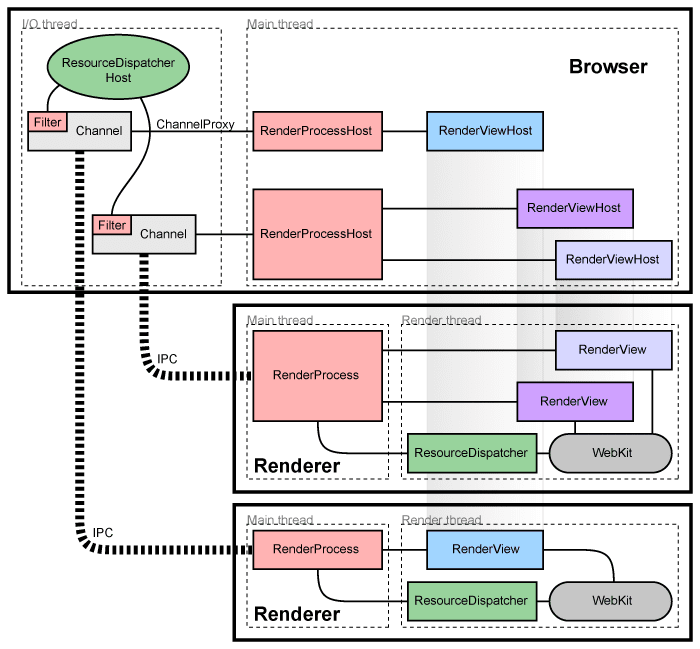
\includegraphics[width=1\columnwidth]{multi-process-arch} 
    \caption{Architettura multi-process in Chrome}
\end{figure}

Il browser crea tre differenti tipi di processi: browser, renderer ed estensioni.

\begin{itemize}
    \item \textbf{Browser}: esiste un unico processo browser, il quale gestisce i tab, le finestre e il browser stesso. Gestisce inoltre tutti i collegamenti delle pagine con il file system, la rete, input utente etc. ma non esegue alcun contenuto delle pagine;
    \item \textbf{Renderer}: il processo browser crea molteplici processi renderer, ognuno responsabile per la visualizzazione di una pagina web. I processi renderer contengono la complessa logica per la gestione di HTML, CSS, JavaScript, immagini e così via. Google Chrome, Safari ed altri utilizzano un rendering engine basato sul progetto open-source WebKit, mentre Firefox ed Edge hanno il proprio;
    \item \textbf{Estensioni}: il processo browser crea anche un processo per ogni estensione
\end{itemize}

\subsection{Strategie multi-process}

Una volta che il browser ha creato il processo omonimo, crea un processo renderer per ogni istanza di pagina web visitata dall'utente. Può essere pensato come un processo separato per ogni tab del browser, ma con l'eccezione di consentire a due tab di convidere lo stesso processo qualora siano collegati tra di loro e mostrino lo stesso sito. \\

Per esempio, se un tab ne apre un altro usando JavaScript o se viene aperto un link verso lo stesso sito in un nuovo tab, questi condivideranno lo stesso processo renderer. Si permette così ai tab correlati di comunicare via JavaScript e condividere la cache. Al contrario, se viene aperta una pagina di un sito diverso verrò riservato un nuovo processo. \\

Per essere precisi, si definisce un "sito" come un dominio registrato (ad esempio google.come o bbc.co.uk) e racchiude anche i sotto-domini (mail.google.com) e le porte (google.com:8080). Un' "istanza di sito" è invece un'insieme di pagine collegate provenienti dallo stesso sito. Due pagine sono considerate connesse se vi sono riferimenti reciproci in codice JavaScript, ad esempio una apre la seconda programmaticamente. Mentre se l'utente digita manualmente lo stesso indirizzo in due tab diverse, vengono considerate due istanze diverse con processi distinti. \\

Di seguito si illustrano nel dettaglio le diverse strategie multi-processi adottati dai browser moderni.

\subsubsection{Process-per-site-instance}

Normalmente i browser usano una strategia "Process-per-site-instance", ovvero lo stesso sito aperto in tab diversi con riferimenti reciproci saranno renderizzati dallo stesso processo. A volte è difatti necessario o desiderabile condividere il processo, quando per esempio un'applicazione web apre una nuova finestra con cui si aspetta di comunicare in maniera sincrona. \\

In generale invece, ogni nuova finestra o tab che non siano lo stesso sito possiede un nuovo processo.

\subsubsection{Process-per-site}

Raggruppa tutte le pagine dello stesso sito nello stesso processo, indipendentemente dalla presenza di riferimenti reciproci. Questa strategia è basata esclusivamente sul dominio del contenuto e non sulle relazioni tra le tab. Di conseguenza può risultare in processi molto onerosi.

\subsubsection{Process-per-tab}

Esiste anche una strategie più semplice che dedica un processo renderer per ogni gruppo di tab. Per ovvi motivi è estremamente inefficiente.

\subsection{Come forzare l'uso di un nuovo processo}\label{forzare-processo}

Dalla descrizione precedente della strategia \textit{Process-per-site-instance}, sembrerebbe non sia possibile ottenere l'effetto desiderato per il progetto \textit{Stargate}. Si desidera difatti alloccare un processo dedicato ad ogni finestra, sebbene appartengano allo stesso sito e quindi contrariamente al comportamento della strategia \textit{Process-per-site-instance}. \\

In seguito a diverse ricerche è tuttavia emerso che è possibile ottenere un processo dedicato come effetto collaterale di un parametro di sicurezza per la creazione delle nuove finestre. Nei browsers moderni è difatti possibile specificare un parametro \texttt{rel=noopener}, che evita exploits di sicurezza in cui la finestra padre è capace di accedere a riferimenti contenuti nella finestra figlia e/o viceversa. 

Quest'ultimo comportamento di condivisione dei riferimento è necessario per il corretto funzionamento di molte applicazioni cross-page, ma pone gli utenti a rischio qualora le nuove finestre siano di dominio diverso e potenzialmente maligne. Tramite il parametro \texttt{rel=noopener} è invece possibile evitare qualsiasi riferimento tra le parti e per, salvaguardare la sicurezza della memoria, ogni finestra creata con tale parametro ha un proprio processo dedicato. \\

Tramite quindi questa funzionalità, la libreria \textit{Stargate} è in grado di forzare un processo per ogni nuova finestra widget. L'altra faccia della medaglia, tuttavia, è la maggior difficoltà di comunicazione tra le finestre in quanto non si possiede più alcun riferimento JavaScript alle finestre. Per tale motivo si sono studiate diverse strategie di comunicazione cross-page, descritte nella prossima sezione.

\section{Comunicazione cross-page}

Nel corso degli anni vi sono state diverse strategie per la comunicazione cross-page tra pagine web in diversi tab, per soddisfare casi d'uso quali fare il check-out in una nuova pagina protetta di PayPal e notificare la pagina principale del risultato. Un altro esempio d'uso è la possibilità di avere una chat in una pagina separata, che tuttavia scambi informazioni con l'applicazione principale. Ed infine ovviamente il caso d'uso in questione, ovvero estrarre componenti UI per i monitor multipli. \\

\subsection{postMessage}

Il metodo \texttt{window.postMessage(message)} permette la comunicazione sicura attraverso istanze di finestre ed altri tipi di oggetti cross-page, ad esempio tra una pagina ed il popup che ha creato.

\texttt{targetWindow.postMessage(message);}

\begin{itemize}
    \item \textbf{targetWindow}: riferimento alla finestra che riceverà il messaggio. Alcuni esempi per ottenere tale riferimento sono:
        \begin{itemize}
            \item \texttt{window.open()} crea una nuova finestra;
            \item \texttt{window.opener} restituisce il riferimento alla finestra genitore che ha aperto la finestra corrente tramite il metodo precendete;
        \end{itemize}
    \item \textbf{message}: dati da inviare all'altra finestra. I dati sono serializzati usando lo \textit{structured clone algorithm} descritto successivamente, ma implica la possibilità di trasmettere una vasta varietà di oggetti in maniera safe senza doverli serializzare;
\end{itemize}

La finestra che riceve il messaggio può rimanere in ascolto attraverso la proprietà JavaScript \texttt{self.onmessage} che assegna alla propria pagina una funzione da invocare ogni volta che arriva un messaggio inviato da \textit{postMessage}.

\begin{lstlisting}[language={[Sharp]C}]
self.onmessage = function(message) {
    // Do something with message
}
\end{lstlisting}

\subsection{Eventi Storage}

Laddove l'API dedicata alla comunicazione cross-page \textit{postMessage} non si possa utilizzare, ad esempio su browsers meno moderni o perché non è possibile ottenere un riferimento alla finestra, è possibile usare gli eventi dello \texttt{Storage}. I browsers forniscono difatti delle API per la lettura e scrittura di dati persistenti anche dopo la chiusura della pagina. Inoltre lo storage è condiviso tra tutte le pagine aventi lo stesso dominio. \\

È quindi dunque possibile usare tali API per comunicare tra le finestre. \\

Esempio di invio di dati:

\begin{lstlisting}[language={[Sharp]C}]
// Salva nel proprio storage, che e' tuttavia condiviso
// tra tab dello stesso dominio
window.localStorage.setItem('stargate-msg', message)
\end{lstlisting}

Esempio di ascolto di dati, ove si rimane in ascolto dell'evento di modifica dello Storage:

\begin{lstlisting}[language={[Sharp]C}]
window.addEventListener('storage', function(event) {
  const message = window.localStorage.getItem('stargate-msg')
})
\end{lstlisting}

È dunque palese che questo metodo sia un trick e non un'API nata allo scopo della comunicazione cross-page, tuttavia è stato utilizzato per anni anche a questo scopo. Un ulteriore aspetto inconveniente di questo approccio è il fatto che sia obbligatorio, a differenza di \textit{postMessage}, serializzare i dati in formato \gls{JSON}. Un confronto tra \textit{structured clone algorithm} e serializzazione è fornito in seguito in questo capitolo.

\subsection{Cookies}

È infine possibile utilizzare i cookies per la comunicazione tra finestre, laddove nemmeno gli eventi \texttt{Storage} siano possibili. La finestra che invia il messaggio lo serializza come stringa e lo scrive all'interno di un cookie del browser. La finestra ricevente è invece in ascolto tramite un timer che ogni tot millisecondi legge il cookie per capire se è stato cambiato. \\

Per diversi motivi quali limiti di dimensione dei cookie, difficoltà di lettura/scrittura, performance e scalabilità è una soluzione assolutamente sconsigliata. \\

Fortunatamente gli obiettivi obbligatori del progetto di stage richiedono il supporto solo di Google Chrome e Firefox, i quali supportano \textit{postMessage}. I browser invece supportati dal prodotto \textit{Route Manager}, ovvero fino ad Internet Explorer 11, supportano almeno gli eventi dello \texttt{Storage}, utilizzabili quindi come fallback.

\subsection{Structured clone algorithm VS Serialization}

Poiché la comunicazione è multi-finestra tra processi separati, è necessario purtroppo che i dati siano copiati da una finestra e l'altra per mantenersi sincronizzati. \\

Lo "Structured clone algorithm" è un algoritmo per la copia di oggetti JavaScript complessi ed è utilizzato internamento per il trasferimento di dati attraverso \textit{postMessage} ed altre API JavaScript. Ciò che fa è realizzare una copia analizzando ricorsivamente l'oggetto input, ma mantenendo una mappa dei riferimenti visitati precedentemente per evitare di attraversare infinitamente strutture circolari. 

Una struttura dati circolare consiste in un campo dell'oggetto il cui valore è il riferimento all'oggetto stesso in maniera diretta (\texttt{a -> a}) o indirettamente (\texttt{a -> b -> a}). \\

Vantaggi dello \textit{Structured clone algorithm}:

\begin{itemize}
    \item Supporto per strutture circolari;
    \item Supporto nativo per la copia di quasi qualsiasi tipo di oggetto JavaScript;
    \item Non vi è bisogno di convertire in un formato e ricostruire l'oggetto originale da tale formato, essendo quindi sia più performante che evitando di rischiare la perdita di informazioni durante la conversione.
\end{itemize}

Svantaggi dello \textit{Structured clone algorithm}:

\begin{itemize}
    \item Non è possibile clonare oggetti \texttt{Error} e \texttt{Function};
    \item Supportato dai browsers che supportano \textit{postMessage}
\end{itemize}

La serialization è invece una tecnica che consiste nel tradurre un oggetto JavaScript in un formato adatto per la trasmissione nelle rete o per il salvataggio. In JavaScript tale formato è una stringa JSON, comune anche ad altri linguaggi lato server.

Vantaggi della \textit{Serialization}:

\begin{itemize}
    \item Adatto per la trasmissione nella rete;
    \item Supportato da qualsiasi browser ed utilizza un formato comune ad altri linguaggi.
\end{itemize}

Svantaggi della \textit{Serialization}:

\begin{itemize}
    \item Non supporta strutture circolari di default;
    \item Supporta solo un sotto-insieme dei tipi di oggetti, in particolare solo i formati definiti dallo standard JSON: numeri, stringhe, booleani, oggetti letterali ed array. Non supporta ad esempio strutture dati quali \texttt{Map, Set, Date, ArrayBuffer}, etc.;
    \item Perdita di informazioni nella conversione oggetto <=> stringa JSON;
    \item Calcolo computazionale per conversione e ricostruzione dell'oggetto originale.
\end{itemize}

\subsection{Conclusioni}

Confrontando le diverse strategie per la comunicazione cross-page e la copia dei dati, è chiaro che la migliore sia l'utilizzo di \textit{postMessage}, il quale sfrutta lo \textit{Structured clone algorithm}. Difatti entrambi sono nati esattamente per uno scopo di comunicazione tra la pagina principale ed altre entità quali estensioni, altre finestre e Web Workers (spiegati in seguito).\\

È invece possibile utilizzare la tecnica degli \textit{Eventi Storage} assieme alla \textit{Serialization} come fallback della libreria \textit{Stargate} qualora il browser di esecuzione non supporti la strategia \textit{postMessage}. Tuttavia a causa delle nette differenze comportamentali tra \textit{Structured clone algorithm} e \textit{Serialization}, gli utilizzatori della libreria sono avvertiti delle possibili complicazioni. Posso quindi decidere se affidarsi al fallback, qualora non utilizzino alcuna struttura dati non supportata dalla \textit{Serialization}, oppure disabilitare l'utilizzo di \textit{Stargate} se il browser non è moderno.\\

Nel caso dell'azienda WorkWave per il prodotto \textit{Route Manager}, è stata decisa proprio la seconda opzione e disattivare l'interfaccia UI che permette di aprire la mappa Google Maps esternamente.

\section{Prima architettura Stargate}

Alla luce delle precedenti informazioni, si illustra di seguito una prima architettura per la libreria \textit{Stargate} e verrà ampliata passo per passo nei prossimi capitoli. Con la strategia \textit{postMessage} è difatti possibile organizzare l'applicazione nel seguente modo, ove si instraura una comunicazione bilaterale in cui \textit{Parent} trasferisce lo stato applicativo ed i vari \textit{Widget} notificano di eventi. \\

\begin{figure}[H] 
  \centering 
  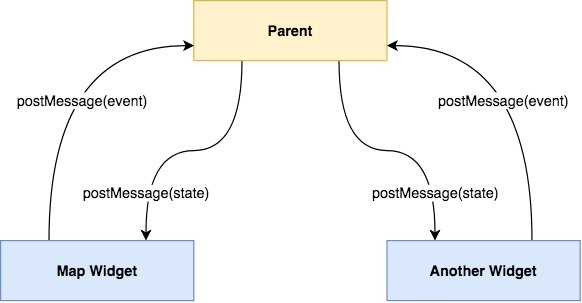
\includegraphics[width=1\columnwidth]{postMessage} 
  \caption{Prima architettura Stargate}
\end{figure}

\textbf{Parent}
    \begin{itemize}
        \item vive nella finestra principale ed è unica per sessione;
        \item si occupa della creazione e comunicazione con le finestre widget, mandando lo stato applicativo dell'applicazione contenente i dati necessari ai vari widget;
        \item gestisce gli eventi dei widget che necessitano di modificare lo stato applicativo dell'applicazione.
    \end{itemize}
\textbf{Widget}
    \begin{itemize}
        \item Vive in una finestra widget, creata dal \textit{Parent}
        \item Riceve lo stato applicativo ed utilizza i dati in essa per la corretta rappresentazione UI. Ogni volta che lo stato cambia, si aggiorna automaticamente anche la UI;
        \item Comunica al \textit{Parent} qualsiasi evento che abbia effetti sullo stato applicativo, ad esempio un'interazione utente.
    \end{itemize}
